% !TeX spellcheck = en_US
\addsection{Units}{\skills/leadership.png}

\begin{multicols*}{2}

\hypertarget{Units}{In}\index{Units} addition to their Hero and its associated deck, players also have \textbf{a deck of Unit Cards} which represent the armies moving with their Heroes.
Every Faction has access to \textbf{7 different Units}, each with unique stats and abilities.
Units are necessary for winning Combat and fulfilling Scenario goals.
Each Scenario's setup instructions indicate which Unit Cards should be included in your initial Unit Deck.
This Deck should be kept clearly separated from the rest of your Faction's Units.\par
Each Faction Unit is double-sided, with a weaker "Few" side, and a stronger "Pack" side.
"Few" units may be upgraded to "Packs" by \textbf{Reinforcing} them, while taking damage can subsequently reduce a Unit back to its "Few" side.
Units should be always kept on their correct side when moved or inspected.\par
A player's Unit Deck may have any number of Units, but \textbf{only up to 5 Units} can be selected to fight during \hyperlink{Combatsetup}{Combat Setup}.
If a Unit is defeated in Combat, \textbf{discard it} from your Unit Deck.\par
Units may be Recruited\index{Recruiting} and Reinforced\index{Reinforcing} by flipping the Population Token\index{Population Token} and paying the Unit's Recruitment \includesvg[height=10px]{\svgs/pay.svg} or Reinforcement \includesvg[height=10px]{\svgs/reinforce.svg} cost.
When you do so, you can instantly Recruit and Reinforce \textbf{any number} of times, provided you have enough Resources and the prerequisite Buildings to do so.\par
\textbf{Recruiting} a Unit requires that your Town has a Dwelling of that Unit's Level (\includesvg[height=10px]{\svgs/bronze.svg}\includesvg[height=10px]{\svgs/silver.svg} \includesvg[height=10px]{\svgs/golden.svg}).
\textbf{Reinforcing} requires that your Town has a Citadel in addition to a Dwelling of that Unit's Level.\par

\note{13}{
  Any effects which instruct you to Reinforce \textbf{do not} require spending your Population Token nor owning a Citadel or any Dwellings.\par

  \medskip

  If all Units in your Unit Deck are defeated, \textbf{immediately} replace your Unit Deck with the starting Units\index{Starting Units} of the Scenario. Defeated Faction Units can always be Recruited again with another use of the Population Token.
}

\vspace*{\fill}
% \hspace{2.62em}
  \hspace{1em}
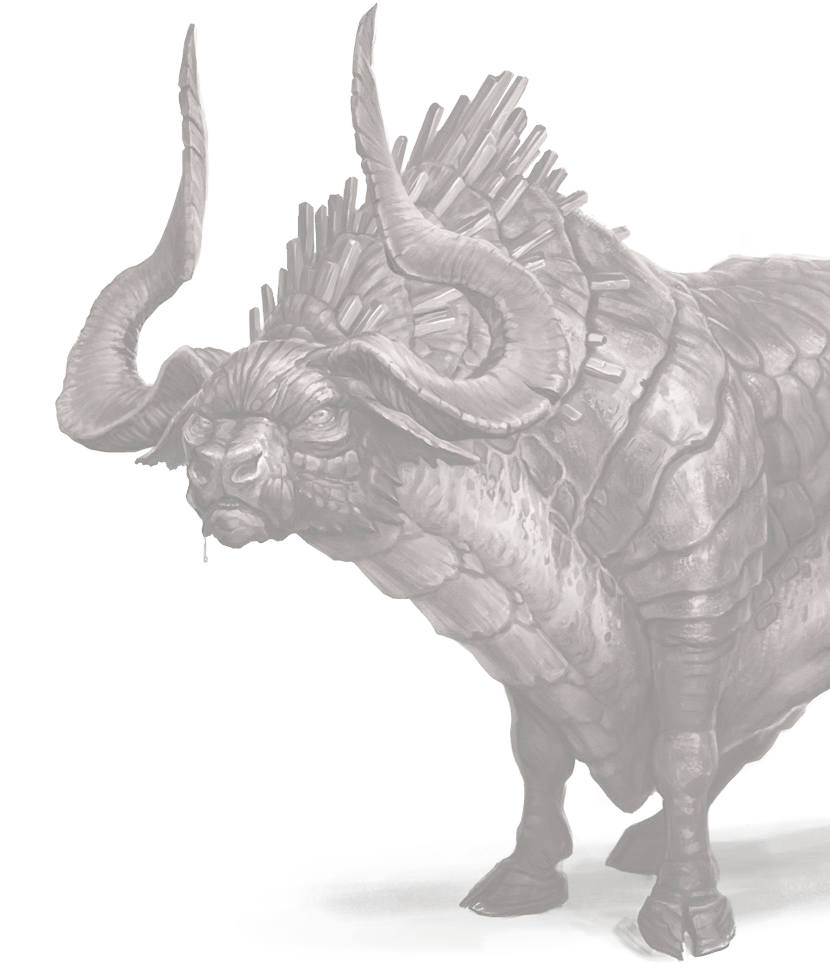
\includegraphics[width=1.2\linewidth]{\art/gorgone.png}

\clearpage

\end{multicols*}
\begin{multicols}{2}
\subsection*{Unit Card Anatomy}

\vspace{0pt}


\includegraphics[height=30px]{\images/attack.png} \textbf{Attack} – The amount of damage this Unit deals when it attacks.\par

\includegraphics[height=30px]{\images/defense.png} \textbf{Defense} - The amount by which this Unit reduces oncoming Attack damage.
Does not apply to damage received from Spells or other non-attack effects.\par

\includegraphics[height=30px]{\images/hp.png} \textbf{\hypertarget{HP}{HP}} - The maximum amount of damage a Unit can sustain before it is defeated.
"Few" Units are discarded from Combat and their owner's Unit Deck when defeated.
"Pack" Units are turned back to "Few" Units, with any excess damage placed on their "Few" side.
Units retain their "Few" or "Pack" status between Combats.
All damage is healed from all Units at the end of Combat.\par

\includegraphics[height=30px]{\images/initiative.png}{\hypertarget{Initiative}{\textbf{Initiative}}} - Determines when the Unit Activates during Combat.
Units with a higher Initiative Activate first.

\vfill
\hspace{-2em}
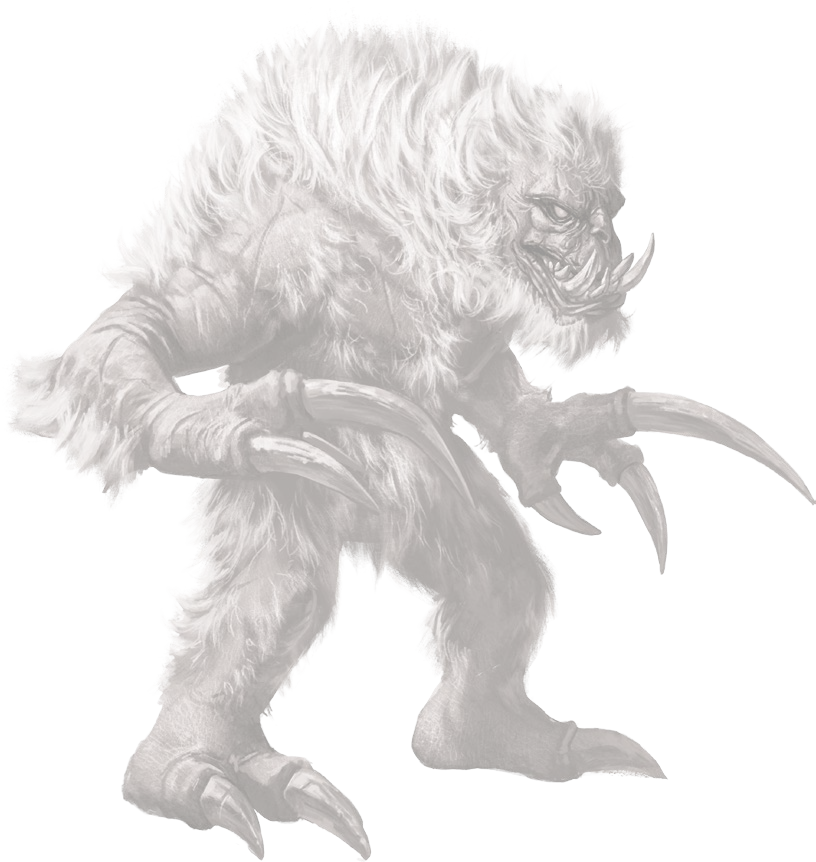
\includegraphics[width=\linewidth]{\art/behemoth.png}

\begin{center}
  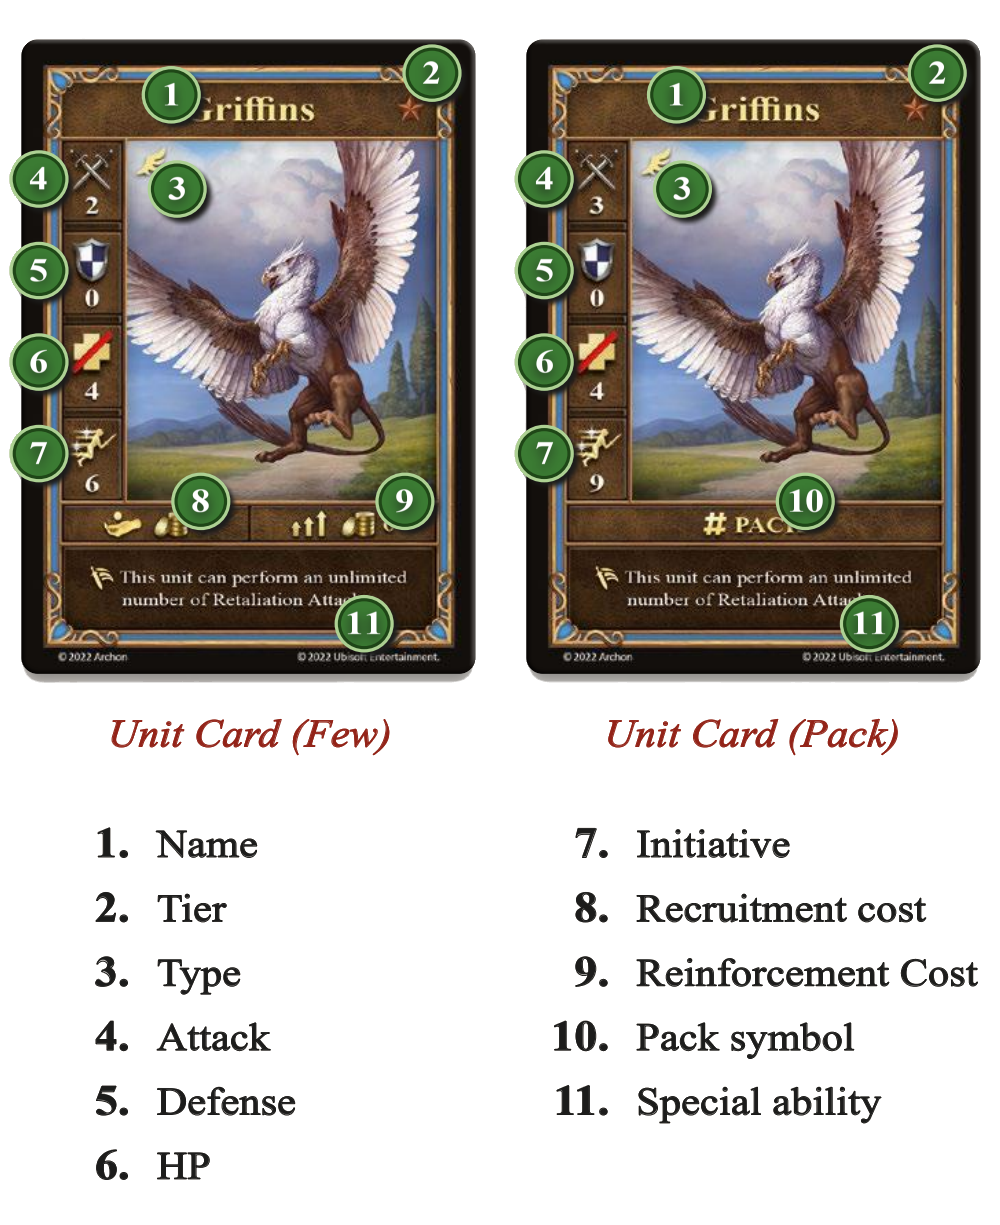
\includegraphics[width=\linewidth]{\cards/units.png}
\end{center}
\vspace{-1em}
\begin{multicols*}{2}
  \footnotesize
  \begin{center}
    \textbf{\textit{\textcolor{darkcandyapplered}{Unit Card (Few)}}}
  \end{center}
  \begin{itemize}
    \item[\textbf{1.}] {Name}
    \item[\textbf{2.}] {Tier}
    \item[\textbf{3.}] {Type}
    \item[\textbf{4.}] {Attack}
    \item[\textbf{5.}] {Defense}
    \item[\textbf{6.}] {HP}
  \end{itemize}
  \columnbreak
  \begin{center}
    \textbf{\textit{\textcolor{darkcandyapplered}{Unit Card (Pack)}}}
  \end{center}
  \begin{itemize}
    \item[\textbf{7.}] {Initiative}
    \item[\textbf{8.}] {Recruitment cost}
    \item[\textbf{9.}] {Reinforcement cost}
    \item[\textbf{10.}]{Pack symbol}
    \item[\textbf{11.}]{Special Ability}
    % \item[\textbf{\phantom{.}}] \phantom{.}
  \end{itemize}
\end{multicols*}

\bigbreak

Most Units have a \textbf{special ability}\index{Special Ability}:\par
\begin{itemize}[wide]
  \item\textbf{Activation} \includesvg[height=10px]{\svgs/activation.svg} resolves when the Unit is Activated.
  \item\textbf{Attack} \includesvg[height=10px]{\svgs/unit_attack.svg} resolves when the Unit attacks during its Activation.
    In case of multiple attacks, resolve the effect for \textbf{the first attack only}.
  \item\textbf{Other} \includesvg[height=10px]{\svgs/unit_other.svg} may be resolved instead of the Unit's normal Activation.
    It replaces all movement and/or attacking.
  \item\textbf{Passive} \includesvg[height=10px]{\svgs/unit_passive.svg} resolves whenever its condition is met.
  \item\textbf{Retaliate} \includesvg[height=10px]{\svgs/unit_retaliate.svg} resolves when the Unit retaliates.
  \item In any other cases without one of the above icons, the Unit's ability is used according to its text.
    Units may also use \hyperlink{Playerdecks}{these} symbols.
\end{itemize}

\vspace*{\fill}

\columnbreak

\subsection*{\hypertarget{Unittype}{Unit Types}}
There are three types of Units:
\begin{itemize}
  \item \textbf{Ground}\index{Ground Units} \includesvg[height=10px]{\svgs/unit_ground.svg} Units may move up to 3 spaces and then attack an adjacent enemy.
  \item \textbf{Flying}\index{Flying Units} \includesvg[height=10px]{\svgs/unit_flying.svg} Units may move up to 3 spaces, \textbf{ignoring Combat Obstacles}, and then attack an adjacent enemy.
  \item \textbf{Ranged}\index{Ranged Units} \includesvg[height=10px]{\svgs/unit_ranged.svg} Units may attack \textbf{any Unit anywhere} and then move up to 1 space OR move up to 1 space without attacking.
\end{itemize}
If a \includesvg[height=10px]{\svgs/unit_ranged.svg} Unit is next to an enemy Unit, its attack target \textbf{must be} that adjacent enemy.
When attacking an adjacent enemy in this way, the \includesvg[height=10px]{\svgs/unit_ranged.svg} Unit suffers a Combat penalty\index{Combat Penalty}: throw two Attack Dice (instead of one) and \textbf{apply the smaller result}.\par
This penalty is also applied if the \includesvg[height=10px]{\svgs/unit_ranged.svg} Unit attacks from its own Backline into the enemy's Backline.
Walls and Gates may also \hyperlink{Walls}{reduce} the damage from  \includesvg[height=10px]{\svgs/unit_ranged.svg} attacks.

\subsection*{Neutral Units}
Neutral Units\index{Neutral Units} guard the various locations on the Game Map.
Starting and winning Combat against them is necessary to Visit most Locations.
Neutral Units are spread into four different tiers, each with their own Deck.
In addition to \includesvg[height=10px]{\svgs/bronze.svg}, \includesvg[height=10px]{\svgs/silver.svg} and \includesvg[height=10px]{\svgs/golden.svg}, there are also Azure \includesvg[height=10px]{\svgs/azure.svg} Neutral Units which are the strongest in the game.\par
Each of these Decks should always be kept separate from each other and shuffled during setup.
If a Neutral Unit Deck ever runs out of Cards, reshuffle the discard into a new Deck.
When a Combat against Neutral Units starts, draw \hyperlink{Difficulty}{the appropriate number} of Units from each tier to take part in that Combat.\par
It is possible for players to gain Neutral Units to their Unit Deck through various effects, such as Scenario-Specific Rules or the Diplomacy Ability Card.
\textbf{Neutral Units cannot be Reinforced}, as they are single sided.
Whenever a Neutral Unit is defeated from anywhere, place it into the appropriate Neutral Discard Pile.\par

\vfill
\hfill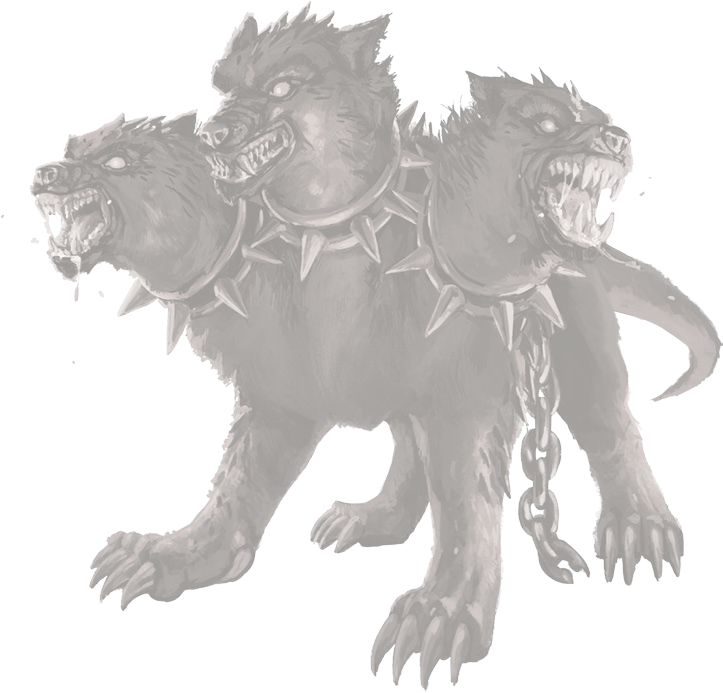
\includegraphics[width=0.7\linewidth]{\art/cerberi.png}

\end{multicols}

\hommtable{14}{
  \begin{tabularx}{\linewidth}{XXXXX}
    & \darkcell{Town Building} & \darkcell{Castle} & \darkcell{Dungeon} & \darkcell{Necropolis} \\
    \darkcell[1.6]{\includesvg[height=12px]{\svgs/bronze-table.svg} \\ Bronze Units} &
      \lightcell[1.6]{Tier 1 \\ Dwelling} &
      \lightcell[1.6]{Halberdiers, Marksmen, Griffins} &
      \lightcell[1.6]{Troglodytes, Harpies, Evil Eyes} &
      \lightcell[1.6]{Skeletons, Zombies, Wraiths} \\
    \darkcell[1.2]{\includesvg[height=12px]{\svgs/silver.svg} \\ Silver Units} &
      \lightcell[1.2]{Tier 2 \\ Dwelling} &
      \lightcell[1.2]{Crusaders, Zealots} &
      \lightcell[1.2]{Medusas, Minotaurs} &
      \lightcell[1.2]{Vampires,\\ Liches} \\
    \darkcell[1.2]{\includesvg[height=12px]{\svgs/golden.svg} \\ Gold Units} &
      \lightcell[1.2]{Tier 3 \\ Dwelling} &
      \lightcell[1.2]{Champions, Archangels} &
      \lightcell[1.2]{Manticores, Black Dragons} &
      \lightcell[1.2]{Dread Knights, Ghost Dragons} \\
  \end{tabularx}
}

\clearpage


\begin{multicols}{2}

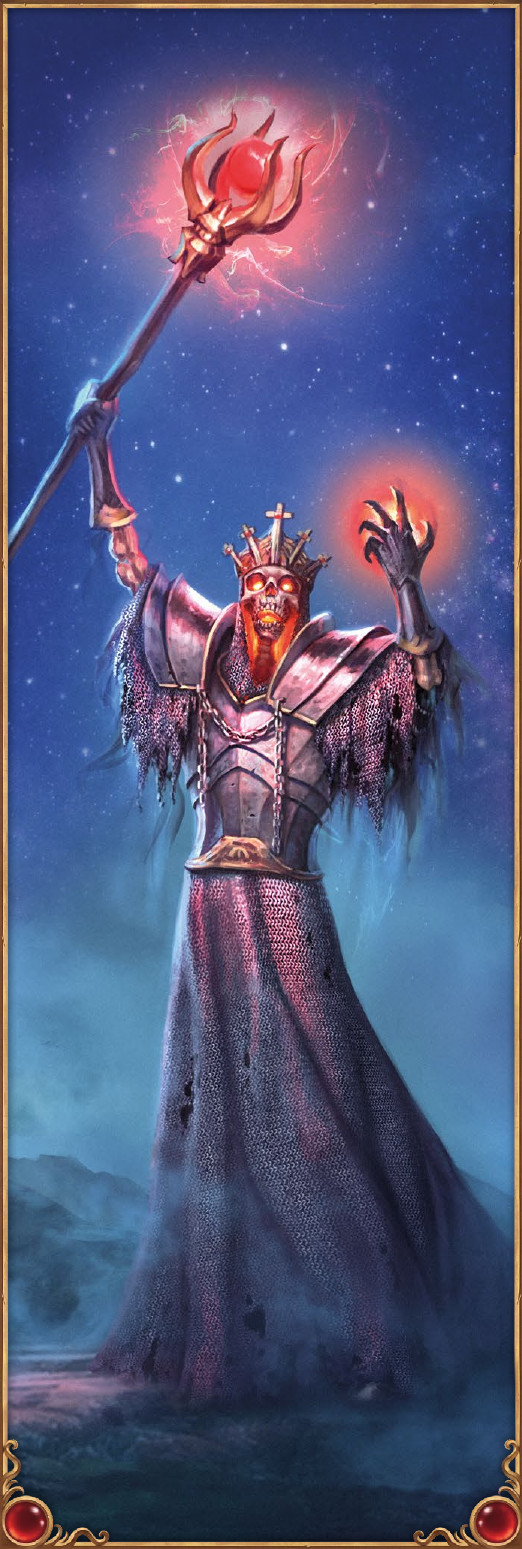
\includegraphics[width=\linewidth]{\art/lich.jpg}

\subsection*{Gameplay Example}

\textit{Bob, playing as Alamar the Warlock, casts a Magic Arrow against Alice's pack of Skeletons, Empowering \includesvg[height=10px]{\svgs/empower.svg} the Spell by 2 with the Expert  Effect \includesvg[height=10px]{\svgs/expert.svg} of a Power Card.}

\medskip

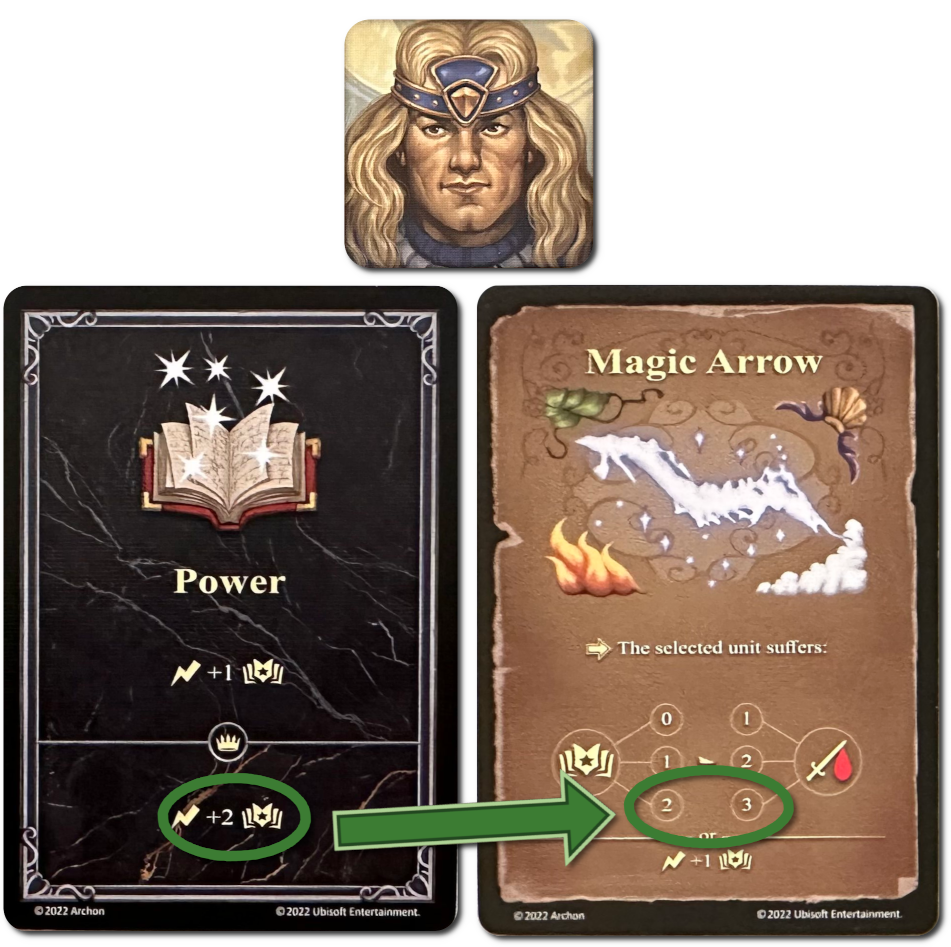
\includegraphics[width=\linewidth]{\examples/alamar_empowering_magic_arrow.png}

\medskip

\textit{The Skeletons take 3 damage \includesvg[height=10px]{\svgs/damage.svg} from the Spell.
  Their Defense \includesvg[height=10px]{\svgs/defense.svg} of 1 does not reduce the damage, because it only applies against attacks.
  The Skeletons have a HP \includesvg[height=10px]{\svgs/health_points.svg} of only 2, so they are now turned to their "Few" side and 1 leftover damage \includesvg[height=10px]{\svgs/damage.svg} is placed on them.
}

\bigskip

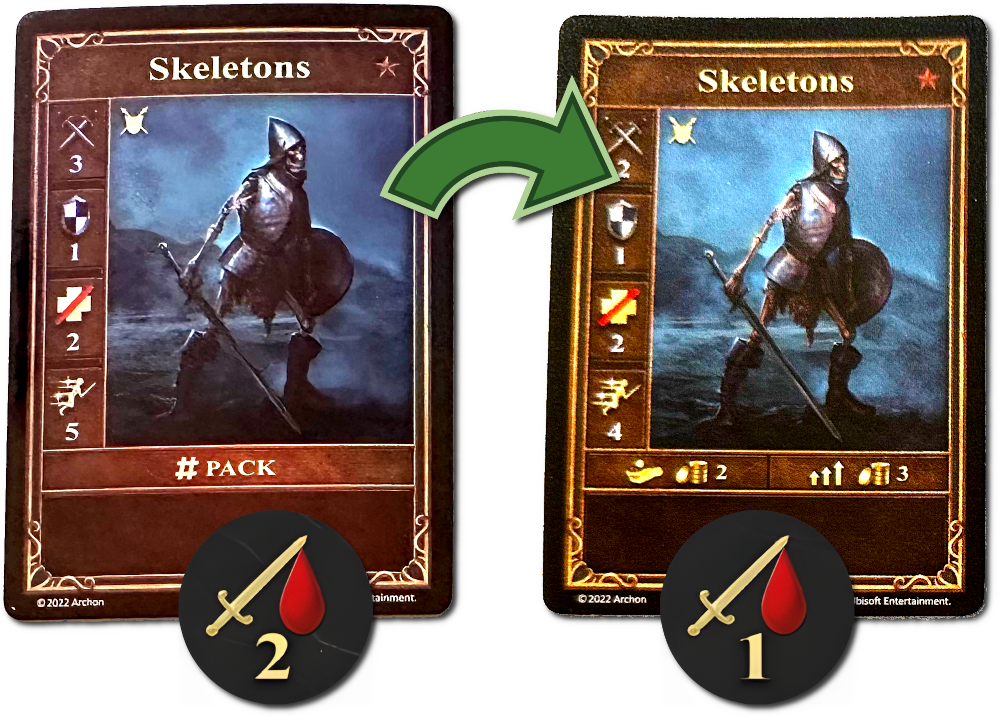
\includegraphics[width=\linewidth]{\examples/skeletons_flipped.png}

\end{multicols}
